\chapter{Sensitivity of a flood-inundation model to rainfall distribution and erosional parameterisation}
\label{chapter_flood_model_sensitivity}
\chaptermark{Flood inundation model sensitivity}
%\begin{refsection}


%\begin{abstract}
%Landscapes evolve and take their shape from the cumulative effect of `geomorphically effective' events. In temperate climates, these are rainfall-driven events of sufficient magnitude to trigger threshold-dependent erosional processes. This chapter investigates the sensitivity of two end-member erosional models to the spatial resolution of rainfall input to a catchment using three historic severe rainfall events in Northern England and Cornwall.
%
%It is demonstrated that the erosional model chosen exerts first-order control of the total amount of landscape change and sediment flux. However, both end member models show sensitivity to the spatial resolution of rainfall input data during individual, formative rainfall events. 
%
%\end{abstract}
\section{Introduction}

Flooding from intense rainfall poses great risk to communities living in proximity to rivers and has the potential to cause loss of life and substantial economic damage in affected areas \citep{pitt2008pitt}. Reliable prediction and advanced warning of flooding requires an understanding of the hydrological processes that operate within a river catchment, in order that operational flood forecasting models may be better parameterised and developed to mitigate against the impact of future events. The interaction of environmental processes within the river catchment system is sensitive to a number of external and internal forcings, including but not limited to precipitation input \citep{nicotina2008impact}, catchment vegetation cover \citep{darby1999effect,andreassian2004waters,bradshaw2007global}, preconditioning of the catchment water table and soil moisture store by antecedent conditions \citep{berthet2009crucial}, urbanisation \citep{hollis1975effect}, debris mobilisation and blockage in river channels \citep{gippel1995environmental,jeffries2003influence}, as well as channel morphological change during flood events \citep{wong2015sensitivity}. 

%Spatial resolution
The question of whether spatial detail in rainfall inputs to a river catchment affects the hydrological response is unresolved, with a number of different studies putting forward seemingly conflicting conclusions. Early studies using deterministic modelling of river catchments and synthetic rainfall fields \citep{wilson1979influence} suggested that detailed space-time representations of rainfall were needed in distributed hydrological models. However, no allusion was made to the possible effects of varying catchment scales. In terms of predicting peak discharge in a catchment \citep{krajewski1991monte}, a small catchment (7.5km\(^2\)), was found to be sensitive to the temporal resolution of rainfall input data, but less so to the spatial distribution of rainfall inputs.  
The role of catchment size is likely to play a part in determining sensitivity to rainfall distribution, with several studies suggesting catchment size can dampen the effect of rainfall spatial variability \citep{segond2007simulation,nicotina2008impact}. The idea of catchment-size dependence has been developed further \citep{gabellani2007propagation}, suggesting that sensitivity to rainfall spatial heterogeneity depends on the characteristic size of the rainfall feature and the catchment size. Systematic investigation of the role of catchment size and morphology have suggested that is specifically the ratio between characteristic hillslope length of the catchment and the rainfall feature that determine sensitivity to spatial heterogeneity \citep{nicotina2008impact}. In cases where the rainfall feature is much greater in size than the typical hillslope length, the effects of rainfall heterogenity on runoff and hydrological response are muted. 

%Morphology change
Understanding how flood dynamics interact with channel and floodplain morphological change is of growing concern for flood modelling \citep{fewtrell2011geometric}. Morphological change during flood events has been shown to be a potential control in the extent of flooding during intense rainfall \citep{wong2015sensitivity}, particularly when river channels undergo geomorphically rapid change during repeated rainfall events of high magnitude \citep{slater2016extent}. Within the context of a single flood, bedload sediment may become highly mobile, and the forces acting on the boundaries of the river channel are sufficient to alter channel geometry in long profile, cross-section, and channel pattern \citep{wong2015sensitivity,kleinhans2013splitting}. As a counterargument, it has ben put forward that during large flood events the floodplain and river channel effectively act as one channel unit, dampening any effects brought about by changes to river channel morphology \citep{bates2005numerical}. The implications of sediment transport and erosion within river catchments has been highlighted as an important factor in flood inundation modelling \citep{lane2007interactions,lane2008reconceptualising,neuhold2009incorporating}, and should form part of an effective flood modelling strategy \citep{wong2015sensitivity} in catchments thought to be sensitive to morphological change during large floods.

% Bring two together.
Flood inundation prediction studies rarely consider both morphological change during flooding or spatial heterogeneity in rainfall inputs to the catchment. Given the reported importance of rainfall resolution on predicting increased sediment yields and channel incision over decades \citep{coulthard2016sensitivity}, can the same observation be made at the time scale of a single event, and does this in turn control the dynamics of a given flash flood event? Though there are differing conclusiions as to importance of rainfall heterogeneity and channel morphological change in flood inundation modelling, there is at least agreement that both have the potential to alter the outcome of flood prediction, under certain conditions. More investigation is needed into which of these uncertainties plays the greater role in determining flood inundation patterns during intense rainfall events and the analysis presented in this chapter attempts to address this by comparing flood inundation model predictions under different rainfall spatial resolution scenarios and erosion law parameterisations. 

%Climate impact etc.
%Growing consensus indicates that intense rainfall events are becoming more frequent in the UK \citep{kendon2014heavier}.

The following questions are explored through the use of numerical modelling experiments set out in Chapter \ref{chapter_events}, Table \ref{table_ensemble_experiments}

\begin{enumerate}
\item Are predicted flood inundation extents during a storm sensitive to the spatial resolution of rainfall inputs to the catchment?
\item Are fluvial erosion and sediment transport controls on predicted flood inundation extents during a single severe storm?
\item Does geomorphic change of the floodplain and channel during a storm event significant enough to affect flood inundation predictions?
\end{enumerate}

%%%%%%%%%%%%%%%%
%\section{Experiment Design \& Method}
%%%%%%%%%%%%%%%%

%\subsection{Rainfall-runoff and flow routing}
%From rainfall input, runoff is calculated using an adaptation of the Beven and Kirby (1979) TOPMODEL. Total surface and subsurface discharge is given by:
%
%\begin{equation}
%Q_{tot} = \frac{m}{T}\log \left( \frac{(r - j_t) + j_t \exp \left( \frac{rT}{m} \right) }{r} \right)
%\end{equation}
%
%where \(T\) is the time step in seconds, \(r\) is the rainfall rate, \(j_t\) is a function that describes soil moisture store, and \(m\) is a parameter that controls the rise and fall of this soil moisture store in \(j_t\). These adapted TOPMODEL equations are given fully in Coulthard (2002), equations (1) and (2).
%
%The amount of water partitioned between surface and subsurface flow is determined by a simple infiltration threshold, given by:
%
%\begin{equation}
%I_t = KS(Dx)^2
%\end{equation}
%
%where \(K\) is hydraulic conductivity, \(S\) is the slope, and \(Dx\) is the width of the grid cell or horizontal grid spacing. The infiltration threshold is subtracted from \(Q_{tot}\) to give the portion of water routed over the surface.
%
%Surface water and channel flow is an important driver in catchment scale erosional processes. The amount and velocity of water flow is a variable in both the sediment transport and bedrock erosion laws. The water flow equations are based on a simplified form of the shallow water flow equations, a simplification first derived by Bates (2010) and incorporated into the landscape evolution model by Coulthard et al (2013). The flow between cells is calculated by:
%
%\begin{equation}
%Q = \frac{q - g h_{flow} \Delta T \frac{\Delta (h+z) }{\Delta x}}{1 + g h_{flow} \Delta t n^2 |q| / h_{flow}^{10/3}} \Delta x
%\end{equation}
%
%where \(q\) is the water flux between cells from the previous iteration, \(g\) is acceleration due to gravity, \(h_{flow}\) is the maximum depth of flow between cells (m), \(t\) is time (s), \(h\) is depth of water, \(z\) is elevation, \(x\) is the grid well width, and \(n\) is Manning's roughness coefficient. The full implementation details are given in Coulthard (2013), and the derivation from the shallow water equations is given in Bates (2010).
%
%\subsection{Sediment transport}
%Transport of loose sediment within the model is governed by the \citet{Wilcock2003} sediment transport model. The Wilcock and Crowe model represents transport of mixed sand/gravel fractions based on the surface sediment composition. The rate of sediment transport, \(q_i\), is given as:
%
%\begin{equation}
%q_i = \frac{F_i {U_*}^3 {W_i}^*}{(s -1) g}
%\end{equation}
%
%where \(F_i\) is the fractional volume of sediment, for a given sediment fraction, \(i\), \(U^*\) is the shear velocity, \(s\) is the ratio of sediment to water density. \({W_i}^*\) is a function relating fractional transport rate to total transport rate (see \citet{Wilcock2003} for a full derivation of this equation). The usage of this sediment transport model is extrapolated here to account for finer particles such as silts \citep{Vandewiel2007}, as well as the sand-gravel mixture it was originally designed for.
%
%\subsection{Bedrock incision}
%\label{bedrock_model}
%A simple model of bedrock incision based on the excess shear stress model (Citations) is implemented in the numerical model. The rate of bedrock incision is determined by the amount of shear stress acting on the bedrock, above a threshold level of stress required to initiate substrate removal (e.g. \citet{Snyder2003}. When bedrock material is removed, it is distributed amongst the sediment fractions according to the fractional proportions set by the user. The rate of bedrock erosion according to the excess shear stress model is given by:
%
%\begin{equation}
%\varepsilon = k_e(\tau_b - \tau_c)^{P_b}
%\end{equation}
%
%where \(k_e\) is the bedrock erodibility coefficient, \(\tau_b\) is the basal shear stress on the channel bed, \(\tau_c\), is the critical shear stress threshold, \(P_b\) is the shear stress exponent. (Cite Howard or Whipple?)

%%%%%%%%%%%%%%%%%%%%%%%%%%%%%
%\subsection{Study area}
%%%%%%%%%%%%%%%%%%%%%%%%%%%%%%
%\subsubsection{Overview}

\section{Sensitivity analysis}
There are numerous user defined parameters in the HAIL-CAESAR model, and in landscape evolution models in general, that have a wide range of potential values. Parameter selection in environmental modelling comes with a degree of uncertainty, and resulting outputs from models can be highly sensitive to the user's choice of input parameters for a given simulation \citep{Pelletier2012}. Initial testing of the HAIL-CAESAR model, and studies using the CAESAR-Lisflood model that it is based upon show it is particularly sensitive to the TOPMODEL \textit{m} parameter, a parameter that controls the rise and fall of the soil moisture store, and hence how a river catchment responds to rainfall input \citep{beven1979physically}. 

To assess the sensitivity of the model to the choice of TOPMODEL-\textit{m} parameter, a series of simulations were carried out with a range of \textit{m} values for both test cases. Simulations of each flood event were carried out with the \textit{m} values shown in table \ref{table-m-sens}.

\begin{table}
\begin{tabular}{lc}
\textbf{Catchment} & \textbf{TOPMODEL \(m\) parameter} \\
\hline
Boscastle   &                                            \\
Ryedale     & 0.03, 0.04, 0.05, 0.06, 0.07, 0.08, 0.09, 0.1, 0.15, 0.2  \\
\hline
\\ 
\end{tabular}
\caption{TOPMODEL \(m\) parameter values used to run sensitivity simulations for each catchment.}
\label{table-m-sens}
\end{table}

%%%%%%%%%%%%%%%%%
\section{Results}
%%%%%%%%%%%%%%%%%

\subsection{TOPMODEL sensitivity}

The model exhibited a strong sensitivity to the choice of the TOPMODEL \( m\) parameter. In the results presented in figure \ref{fig_topmodel_m_ryedale} peak river discharge ranged from XX at an \(m\) value of 0.003 to XX with an \(m\) value of 0.008. The measured peak discharge reported for the 2005 storm at the Ness gauging station was 105 cumecs. In the sensitivity simulations, a value of \(m = 0.005\) produced a flood peak most closely matching the observed value, peaking at XX cumecs (Note the time as well.). 

There were differences between the hydrographs of the observed and simulated discharges in terms of peak discharge timing and recession limb shape. The observed hydrograph showed a sharp rise at around 50 hours after the start of the simulation period. Lower \(m\) values (m \textless 0.005) resulted in a prediction of the flood peak being too early compared to the observed timing, with values \textgreater \ 0.005 predicting the flood peak timing too late. Most of the simulations failed to capture the extended duration of peak discharge, which lasted approximately 5--6 hours, before receding back to low flow levels. The simulation with \(m = 0.006\) came closest to predicting this hydrograph shape, but failed to predict the magnitude of water discharge correctly, underestimating the peak flow by almost 50\%. 

For Ryedale simulations, it was decided to use an \(m\) value of 0.005, providing the closest possible match to the flood peak discharge, though not the true shape of the hydrograph and the receeding limb. As the catchment simulations include a representation of erosion and sediment transport processes, which are often threshold dependent, it was felt necessary to match the discharge peak more closely over choosing to match the hydrograph shape precisely.

\begin{figure}[t]
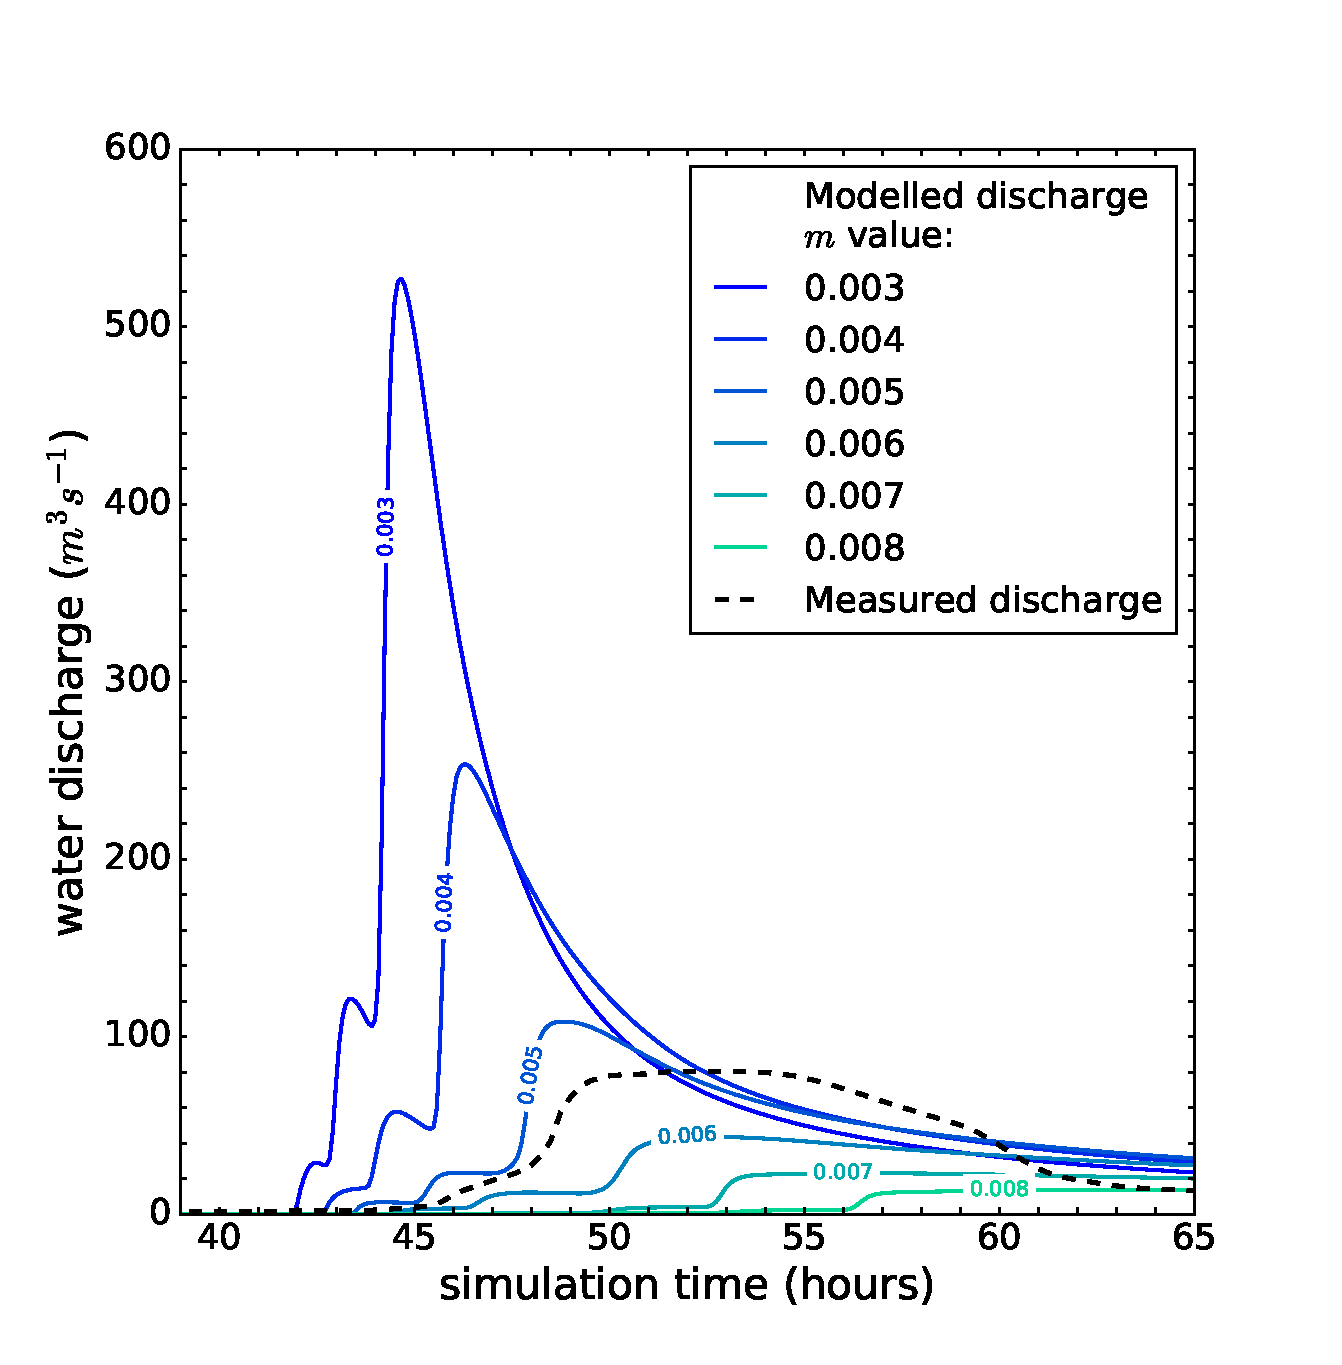
\includegraphics[width=11cm]{chp06_figures_scripts/figure_ryedale_M_sens.eps}
\caption{Discharge at Ryedale catchment outlet for varying values of the TOPMODEL \(m\) parameter. The measured discharge at the catchment gauging station is overlain in dashed line. The results from the simulations with \(m\) \textgreater \ 0.008 are omitted for clarity due to the low peak discharges they produced.}
\label{fig_topmodel_m_ryedale}
\end{figure}

\subsection{Catchment hydrology}

%Comparisons with the actual hydrographs from the gauged basins?

At the catchment scale, hydrological response was sensitive to both the rainfall resolution and the choice of erosional model. For both catchments, higher resolution rainfall input data resulted in a greater maximum river discharge. In the Ryedale experiments, simulations using the gridded rainfall input experienced a flashier hydrological response, reaching peak discharge several hours before the uniform rainfall input cases. This was not observed in any of the Boscastle simulations, with all simulations reaching peak discharge within 30 minutes of each other.

The choice of erosion model also influenced the hydrological response. When catchment erosion was modelled using a transport-limited case, peak discharges were higher in all cases, but the timing of hydrograph peaks remained similar for each case. The difference in peak discharges were minimal when comparing the detachment-limited cases to the hydrological-only models.

\begin{figure}[t]
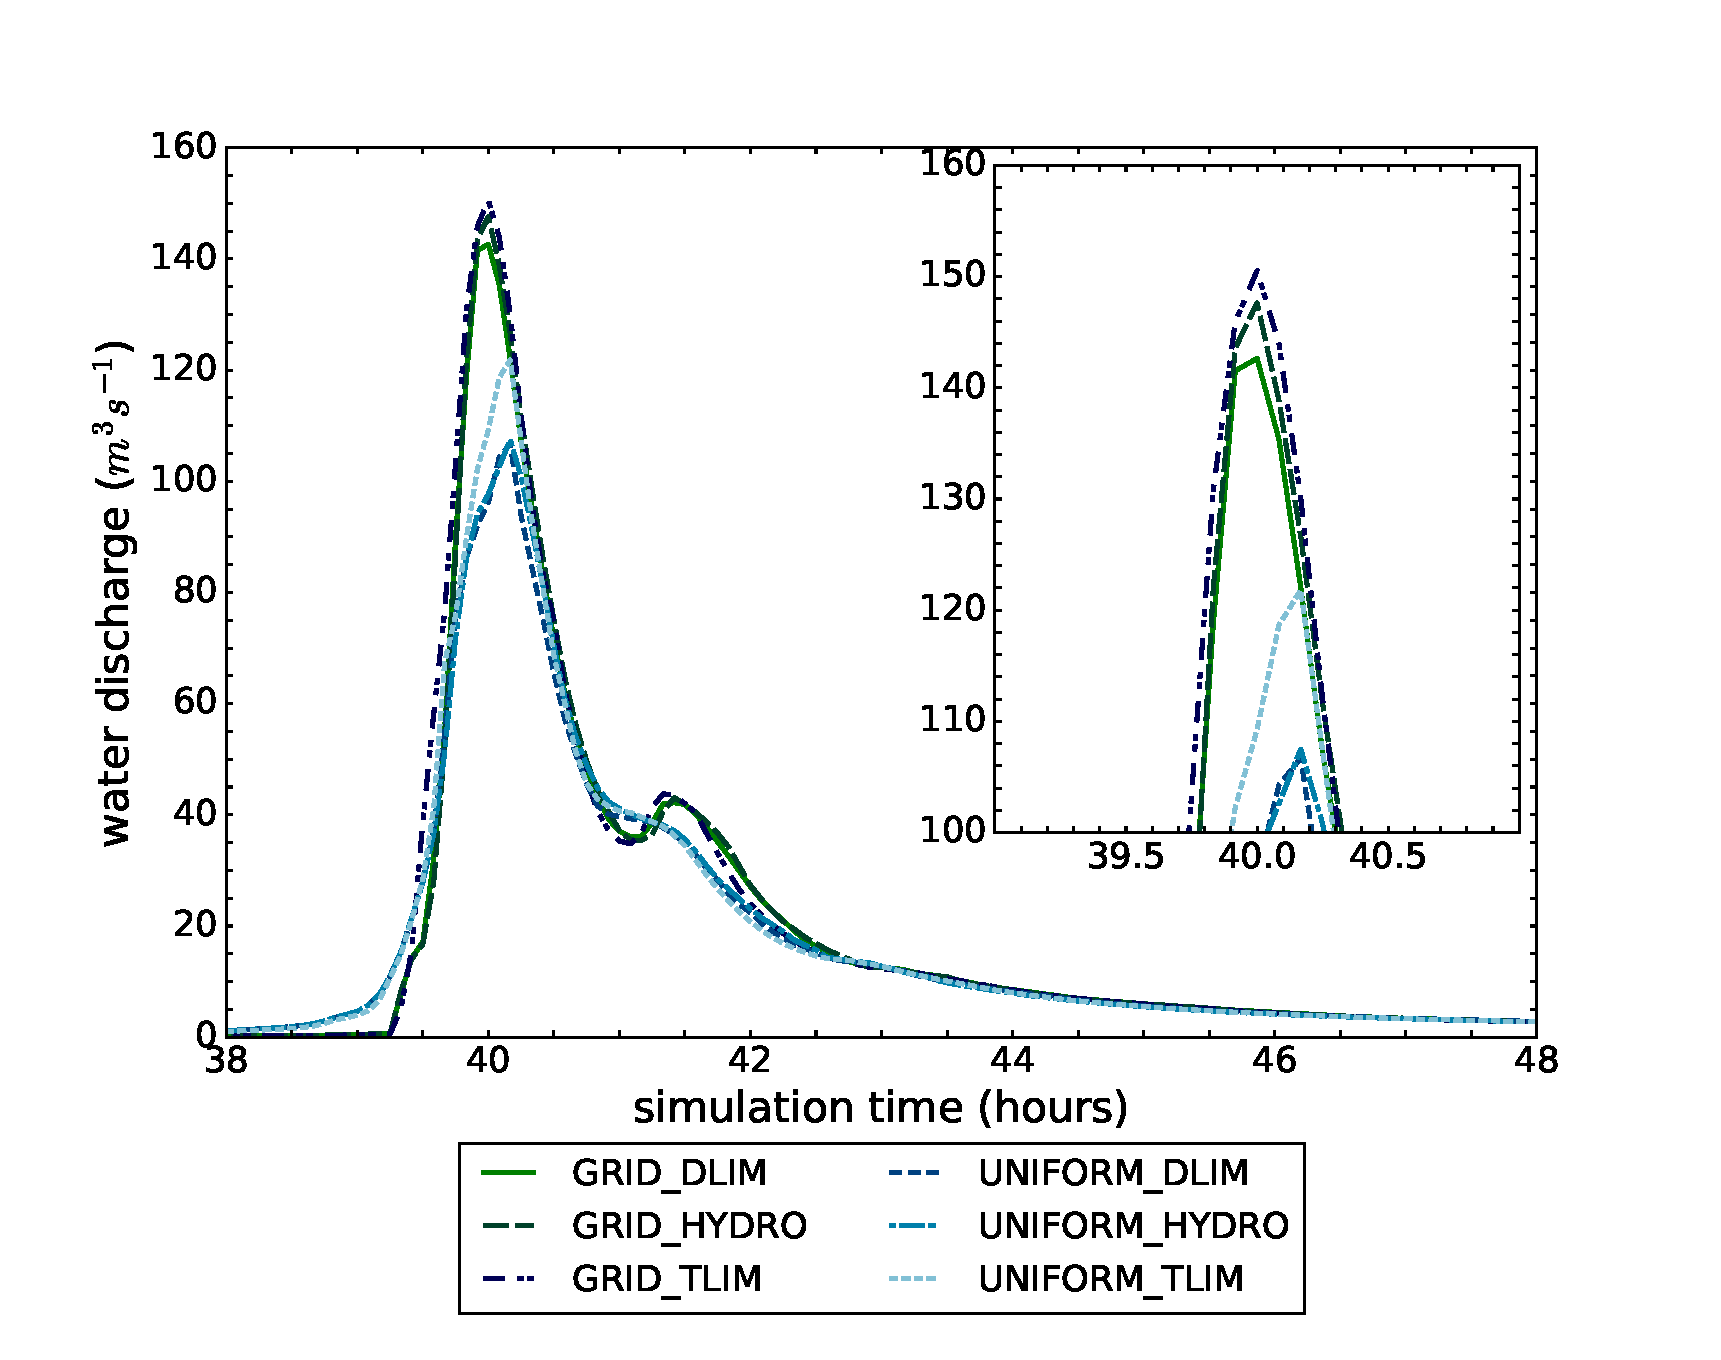
\includegraphics[width=14cm]{chp06_figures_scripts/figure_boscastle_hydrograph_ensemble.eps}
\caption{Boscastle hydrographs (discharge over time at catchment outlet) for each simulation of the 2004 Boscastle event listed in Table \ref{table_ensemble_experiments}. Inset shows detail of main flood peaks around hour 40 of the simulation.}
\label{fig_boscastle_hydrograph_ensemble}
\end{figure}

\begin{figure}[t]
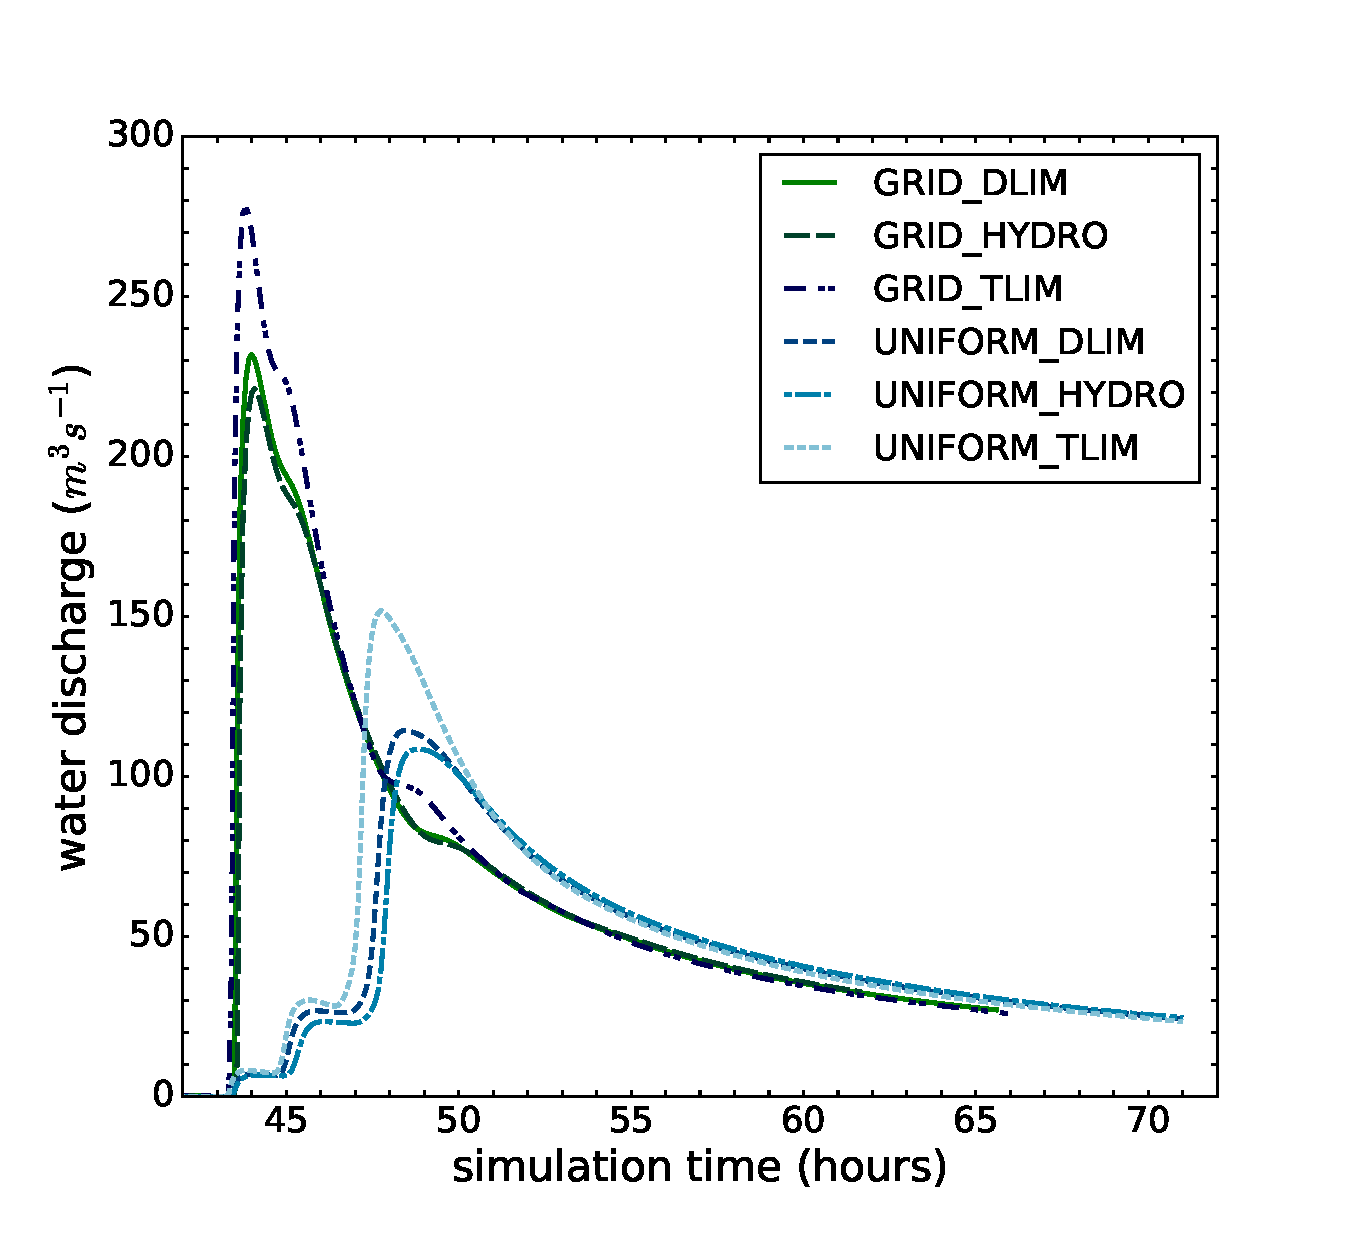
\includegraphics[width=14cm]{chp06_figures_scripts/figure_ryedale_hydrograph_ensemble.eps}
\caption{Ryedale hydrographs (discharge over time at catchment outlet) for each simulation of the 2005 Ryedale event listed in Table \ref{table_ensemble_experiments}.}
\label{fig_ryedale_hydrograph_ensemble}
\end{figure}



\subsection{Spatial variation in flood inundation}
\subsubsection{Boscastle}
The Boscastle catchment simulations showed minimal variation in flood inundation extent. Simulations with gridded rainfall input did not result in substantially different predictions of floodwater inundation compared to those with uniform rainfall input. Both sets of simulations reflected the general extent of reported flood water extents \citep{wallingford2005flooding}. Simulations that allowed erosion to take place (GRID\_TLIM and UNIFORM\_TLIM) showed a slight difference in the variation of floodwater depths in the floodplain area, particularly in the vicinity of Boscastle village, where Figure \ref{fig_boscastle_2dplan_flood_ensemble} is centred on. In hydrological-only simulations, the deepest water depths were predicted to occur in the confines of the river channel, whereas in erosion-enabled simulation, there appeared to be a `smoothing' effect of water depths between the channel and the adjacent floodplain, suggesting that the channel geometry had altered during the flood event either by infilling from sediment from upstream or collapse of the adjacent river banks. Engineer's reports of the Boscastle flood noted that the river channel in the Boscastle village area had indeed been inundated with debris during the storm, which had potentially contributed to the extent of the flooding within the village.

\subsubsection{Ryedale}
The Ryedale simulations showed greater variation in flood extent between the gridded rainfall and uniform rainfall inputs. The flood extents were greater in the gridded rainfall input simulations, corresponding with the higher peak discharges predicted in these simulations.  The variation in water depths appeared to be less sensitive in comparison to the Boscastle simulations. In the lower reaches of the catchment (Figure \ref{fig_ryedale_2dplan_flood_ensemble}, there appeared to be little indication that flood extents or water depths were sensitive to the erosion parameterisation, in contrast to the Boscastle simulations.



% Plan view erosion diff maps
\begin{sidewaysfigure}[t]
\includegraphics[width=20cm]{chp06_figures_scripts/figure_boscastle_peak_flood_ensemble.png}
\caption{Flood extents in the Boscastle catchment at the time of maximum river discharge for each simulation.}
\label{fig_boscastle_2dplan_flood_ensemble}
\end{sidewaysfigure}

% Plan view erosion diff maps
\begin{sidewaysfigure}[t]
\includegraphics[width=20cm]{chp06_figures_scripts/figure_ryedale_peak_flood_ensemble.png}
\caption{Flood extents in the Ryedale catchment at the time of maximum river discharge for each simulation.}
\label{fig_ryedale_2dplan_flood_ensemble}
\end{sidewaysfigure}



\section{Discussion}

The size of the two catchments appears to be a determining factor in how sensitive hydrogeomorphic processes are to the rainfall data input resolution. The Boscastle catchment at 18 km\(^2\) is approximately an order of magnitude smaller than the Rydedale catchment at 270 km\(^2\). For each simulation using gridded rainfall input, the cell width of the rainfall grid is 1 km. The relative amount of increase in rainfall detail between uniform and gridded simulations is much greater in the larger Ryedale catchment than the Boscastle catchment. By using a 1 km gridded rainfall product as input data, the Ryedale simulation potentially captures 15 times more rainfall heterogeneity compared to the respective Boscastle simulation, by virtue of it simply being a much larger catchment with a greater number of rainfall input cells. Catchment size is known to be a factor in hydrological studies of rainfall resolution, and larger catchments are reported to show greater sensitivity to rainfall resolution \citep[e.g.][]{nicotina2008impact}, in terms of hydrological response.

Increasing the resolution of rainfall input data may not be enough to observe sensitivity in smaller catchments, as rainfall features themselves may not exhibit the necessary heterogeneity in structure to benefit from being resolved at finer scale. Rain cells or bands equal to or greater in size than the catchment over which they rain upon, may well be homogeneous enough in spatial extent and rainfall rate that a `uniform' approximation of their rainfall rate is sufficiently precise enough to represent the rainfall rate at all points in the catchment. As seen in the Boscastle catchment simulations, using a detailed rainfall input data source did not notably alter the outcome of the hydrological predictions (Figures \ref{fig_boscastle_2dplan_flood_ensemble}, \ref{fig_ryedale_2dplan_flood_ensemble}). In the Ryedale catchment simulations, the hydrological predictions were notably different based on the choice of rainfall input data resolution, affecting both the time and magnitude of the resulting flood peak. 

Talk about size of convective cell features. What is typical storm cell size and heterogeneity (decay from centre?).


%%%%%%%%%%%%%%%%%%%%%
\section{Conclusions}  %% \conclusions[modified heading if necessary]
%%%%%%%%%%%%%%%%%%%%%
Catchment hydrological response on the short term scale -- such as during the course of single storm event -- is also sensitive the spatial input pattern of rainfall, with the simulations carried out in this study also supporting similar work of \citep{nicotina2008impact} AND OTHERS.

%\printbibliography
%\end{refsection}
